\newpage
\section[federated]{Federated Learning}

W tym rozdziale przedstawiony zastany projekt systemu, który korzystając z podejścia Federated  Learning (FL) umożliwi na trening ekstraktora cech twarzy w rozproszonym środowisku urządzeń IoT.


\paragraph{Federated Learning}

Federated Learning (FL) jest podejściem zastosowania uczenia maszynowego w rozproszonym
środowisku pozwalające na trening modeli on dużym zbiorze danym zdecentralizowanych prywatnych
danych znajdujących się na urządzeniach końcowych użytkowników, a w szczególności urządzeniach
Internetu Rzeczy. FL realizuje ideę "przyniesienie kodu do danych, zamiast danych do kodu" i
adresuje fundamentalne problemu prywatności, własności i lokalności danych. Federated learning
został opisany w (cite).
Problemy odpowiednie do zastosowania federated learningu moją następujące właściwości:
\begin{itemize}
\item Trening na rzeczywistych danych gromadzonych na urządzaniach mobilnych dają znaczą przewagę
nad treningiem na ogólnie dostępnych danych proxy dostępnych w centrach danych.
\item Te dane są prywatne albo są zbyt duże do przetrzymywania ich w centrach danych
\item Dla zadań nadzorowanych, etykiety danych powstają samoistnie z interakcji użytkownika z urządzeniem.
\end{itemize}

\paragraph{Cechy środowiska systemu}

Algorytmy optymalizacji mogące być zastosowane do optymalizacji na urządzaniach IoT mają kilka cech wyróżniających je od znanych już algorytmów rozproszonej optymalizacji:
\begin{itemize}

\item \textbf{Non-IID} Dane trenujące on danym urządzaniu są zazwyczaj zależne od konkretnego użytkownika i dlatego lokalny zbiór danych zebrany na dowolnym urządzeniu nie będzie reprezentatywny w stosunku do dystrybucji całej populacji
\item \textbf{Niezbalansowany} Podobnie, niektórzy użytkownicy będą o wiele częściej korzystali z aplikacji aparatu niż inni, co będzie prowadziło do różnic w wielkości zebranych lokalnych zbiorów  danych trenujących.
\item \textbf{Masywnie rozproszony} Spodziewa się, że liczba finalnych użytkowników biorąca udział w optymalizacji będzie większa niż średnia liczba przykładów trenujących przypadająca na jednego klienta.
\item \textbf{Ograniczona komunikacja} Urządzania IoT są pomimo założenia, że mają dostęp do
internetu mogą być ograniczone wolnym albo kosztownym łączem sieciowym.
\end{itemize}

W tej pracy główna uwaga zostanie poświęcona na doprowadzenie systemu do działania w patologicznym przypadku środowisku danych Non-IID oraz ograniczonej i zawodnej komunikacji.


\subsection{Projekt systemu}

Implementowany system umożliwia trening głębokich sieci neuronowych on danych przetrzymywanych na
bezpośrednio urządzaniu IoT. Dane te nigdy nie opuszczają samego urządzania. Wagi modelu są
agregowane i łączone na serwerze znajdującym się w chmurze za pomocą algorytmu Federated
Averaging konstruując nowy model globalny, który zostaje przesłany z powrotem do urządzeń końcowych
do inferencji. System ten został opisany pierwotnie w (cytat) i z sukcesem zaaplikowany w
implementacji inteligentnej klawiatury smartphone. (cite blogaska googla).


Przedstawienie architektury systemu zaczynamy od przedstawienia protokołu według, którego przebiega cały przepływ danych. Opisujemy to w następnej sekcji.

\subsubsection{Protokół}

Uczestnikami protokołu są urządzania Internetu Rzeczy oraz serwer, który jest usługą chmurową.
Urządzania anonsują serwerowi swoją gotowość do uruchomienia zadania. Zadanie jest specyficzne dla populacji urządzeń i polega na lokalnym uruchomieniu obliczeń, takich jak trening z zadanymi przez serwer parametrami albo ewaluacja wytrenowanego modelu na lokalnych dla urządzenia danych.

Protokół dzieli komunikacje na rundy, z której każda zaczyna się od selekcji. Z potencjalnie tysięcy gotowych urządzeń w danym oknie czasowym, serwer wybiera ich podzbiór, który dostanie zaproszenia do wzięcia udziału obliczeniach. Liczebność tego podzbioru jest parametrem algorytmu opisywanego w kolejnym rozdziale

Serwer mówi wybranym urządzeniom jakiego typu obliczenia będą wykonywane. Wraz z tą informacją
przesłany graf obliczeniowy modelu, zserializowane parametry globalnego modelu oraz pozostałe
informacje niezbędne do uruchomienia obliczeń w danej rundzie. Następnie każdy z uczestników  wykonuje lokalnie obliczenia bazując na globalnym stanie oraz swoim lokalnym zbiorze danych i przesyła wynik obliczeń z powrotem na serwer. W szczególności wynikiem, w przypadku rundy treningowej, będą wytrenowane parametry modelu lokalnego. Serwer wciela zebrane aktualizacje w swój stan globalny co kończy pojedyńczą rundę i proces ten się powtarza.

Opisywany protokół pozwala urządzeniom końcowym na poprawianie globalnego, pojedyńczego modelu pomiędzy rundami, z których każda składa się z trzech faz co zostało pokazane na rysunku (rysunek?).

\paragraph{Selekcja}
Cyklicznie, urządzenia, które spełniają wymagane kryteria (Patrz sekcja XXX) meldują serwerowi swoją gotowość. Serwer wybiera podzbiór z dostępnych mu urządzeń. W naszej implementacji wybrano prostą, losową selekcje  z rozkładem jednostajnym \(N\) urządzeń z tych, które
ogłosiły swoją gotowość. 


\paragraph{Konfiguracja}
Serwer jest skonfigurowany na podstawie wybranego mechanizmu selekcji urządzeń oraz agregacji
modeli. Urządzenia końcowe są samo-konfigurowane według przesłanej przez serwer informacji o typie obliczeń, grafu obliczeniowego oraz stanu globalnego.

\paragraph{Raportowanie}
Serwer czeka, aż partycypujące urządzenia zdadzą raport z wynikiem przeprowadzonych obliczeń. Jeśli runda była rundą treningową to wraz z otrzymaniem wszystkich zaktualizowanych modeli, serwer agreguje je z użyciem algorytmu Federated Averaging i informuje raportujące urządzenia kiedy mogą ponownie zgłosić swoją gotowość. Jeśli wystarczająca liczba urządzeń zaraportuje wyniki serwerowi w pewnym oknie czasowym, runda zostanie uznana za zakończoną z powodzeniem i zagregowany model zastąpi aktualny model globalny. W przeciwnym przypadku zebrane wyniki z tej rundy zostają porzucone. Protokół jest w pewnym stopniu odporny na to, że partycypujące urządzenia z pewnych powodów nie odpowiedzą na przesłaną konfiguracje albo nie zaraportują wyników.

Fazy selekcji i raportowania są dospecyfikowane przez zestaw parametrów. Podczas fazy selekcji  serwer bierze pod uwagę pożądaną liczbę uczestników rundy, czasy time-outów oraz minimalną liczbę potrzebnych uczestników do rozpoczęcia rundy. Faza selekcji trwa dopóty dopóki nie zostanie wybrana docelowa liczba urządzeń albo nie skończy się czas przeznaczony na faze selekcji. W drugim przypadku runda zostanie rozpoczęta jeśli została zebrana minimalna liczba urządzeń, w przeciwnym przypadku runda zostaje porzucona. Faza raportowania parametryzowana jest przez minimalną liczbę urządzeń, które muszą zaraportować wynik.

\subsubsection{Urządzenie IoT}


\subsubsection{Serwer}


\subsection{Algorytm optymalizacji}

  \begin{polishalgorithm}[t]
    \begin{algorithmic}
    \SUB{Server executes:}
      \STATE{} initialize $w_0$
      \FOR{each round $t = 1, 2, \dots$}
        \STATE{} $m \leftarrow \max(\clientfrac\cdot K, 1)$
        \STATE{} $S_t \leftarrow$ (random set of $m$ clients)
        \FOR{each client $k \in S_t$ \textbf{in parallel}}
          \STATE{} $w_{t+1}^k \leftarrow \text{ClientUpdate}(k, w_t)$ 
        \ENDFOR{}
        \STATE{} $w_{t+1} \leftarrow \sum_{k=1}^\nc \frac{n_k}{n} w_{t+1}^k$
      \ENDFOR{}
      \STATE{}
    
    \SUB{ClientUpdate ($k, w$):}\ \ \  // \emph{Run on client $k$}
      \STATE{} $\mathcal{B} \leftarrow$ (split $\pp_k$ into batches of size $\lbs$)
      \FOR{each local epoch $i$ from $1$ to $\lepochs$}
        \FOR{batch $b \in \mathcal{B}$}
          \STATE{} $w \leftarrow w - \eta \grad \loss(w; b)$
        \ENDFOR{}
    \ENDFOR{}
    \STATE{} return $w$ to server
    \end{algorithmic}
    \mycaptionof{algorithm}{\fedavglong. The $\nc$
      clients are indexed by $k$; $\lbs$ is the local minibatch size,
      $\lepochs$ is the number of local epochs, and $\eta$ is the learning
      rate.}\label{alg:fedavg}
    \end{polishalgorithm}


  Algorytm~\ref{alg:fedavg} opisany został zaimplementowany w języku Python. Do implementacji modeli
  neuronowych i algorytmów uczących został wykorzystany framework
  PyTorch~\cite{paszke2017automatic}. Poprawność implementacji została sprawdzona na zadaniu klasyfikacji obrazów wykorzystując prostą sieć konwolucyjną oraz popularny zbiór danych CIFAR10. 

  \paragraph{Sieć konwolucyjna}

  Jako obiekt treningu omawianego algorytmu zastała użyta niewielka sieć neuronowa zawierająca
  dwie warstwy konwolucyjną z filtrami o szerokości 5x5 (pierwsza z 32 kanałami, druga z 64, po
  każdej dodatkowa warstwa 2x2 max pooling), po których następuje dwu-warstwowy perceptron i na
  końcu warstwa przekształcenia liniowego, co daje w sumie \(10^6\) miliona parametrów. Model został podsumowany w tabeli 


  \paragraph{CIFAR10}

  CIFAR10 jest popularnym syntetycznym zbiorem danych. Zbiór danych składa się z \(\num{60000}\)
  kolorowych obrazów podzielonych na \(\num{10}\) klas, z \(\num{6000}\) obrazami przypadającymi
  na jedną klasę. Zawarte są w nim obrazy o szerokości i wysokości 32 pikseli. Standordowo zbiór
  dzieli się na dwa zbalansowane klasowo podzbiory: testowy i treningowy zawierających odpowiednio
  \(10000\) i \(50000\) etykietowanych przykładów. Na rysunku~\ref{fig:cifar10_example} znajduje się 10 losowo wybranych obrazów, dla każdej z 10 klas.

  \begin{figure}[t]
    \centering
    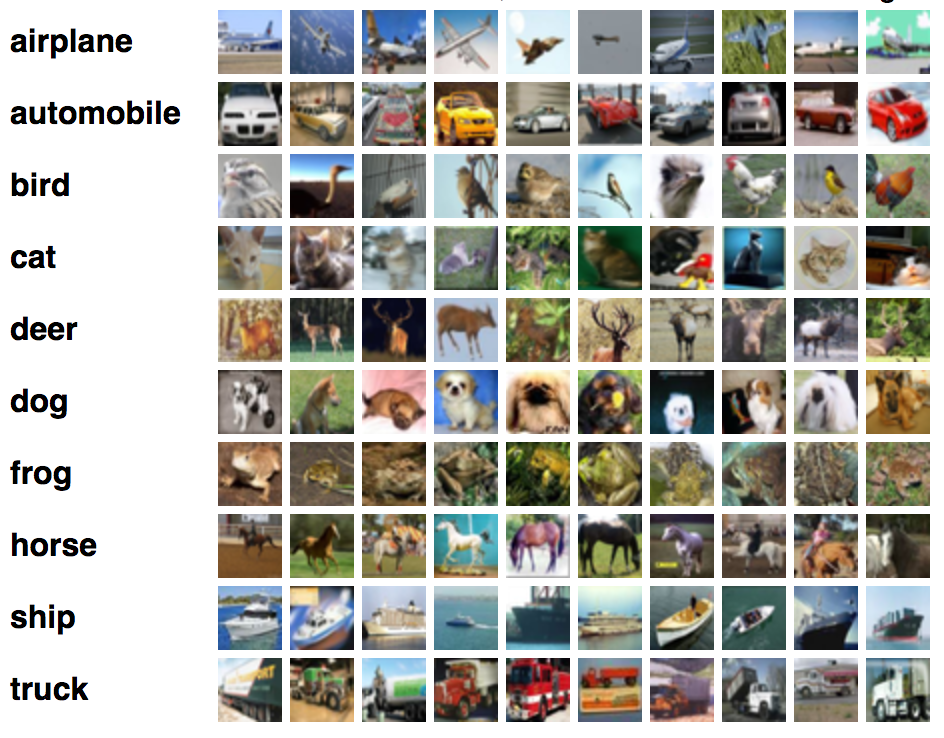
\includegraphics[width=1.0\textwidth]{img/cifar10_example.png}
    \mycaptionof{figure}{10 przykładowych obrazów dla każdej z \(\num{10}\) klas zbioru CIFAR10}
    \label{fig:cifar10_example}
  \end{figure}

  \paragraph{Protokół treningowy}

  Do sprawdzenia poprawności implementacji została zaimplementowana procedura treningowa wzorowana
  na~\cite{mcmahan2016communicationefficient}. Zbiór treningowy został podzielony pomiędzy 100 użytkowników tak żeby każdy zawierał po 500 przykładów trenujących. Z powodu braku naturalnego podziału danych na tak dużą liczbę klientów rozważany jest tutaj nieco mniej wymagający przypadek, w którym dane każdego użytkowania są zbalansowane oraz równomiernie rozdystrybuowane.

  Naszym celem była maksymalizacja dokładności z jaką model klasyfikował obrazy pochodzące ze
  zbioru testowego.Badanie jakości końcowego modelu globalnego odbywało się już nie w sposób
  rozproszony, a na serwerze stosując cały dostępny zbiór testowy, co zostało umożliwione dzięki wprowadzonym uproszczeniom co do rozkładu danych.

  Obrazy uległy standardowemu przetworzeniu wstępnemu i augmentacji. Przykłady trenujące zredukowano do wielkości 24x24 pikseli przez losowe obcięcie krawędzi, obrazy uległy losowemu horyzontalnemu odbiciu lustrzanemu  oraz standardowej normalizacji.

  Zaimplementowany algorytm został porównany do standardowego algorytmu SGD (cytat).


  \paragraph{Ewaluacja}